\chapter{Entwicklung eines GraphQL-Service in .NET mit HotChocolate}
In diesem Kapitel wird die Entwicklung des Prototypen beschrieben.
Der Prototyp ist ein GraphQL-Service welcher mit .NET 6 und der Zuhilfenahme der Bibilothek HotChocolate entwickelt wurde.
Desweiteren wird auf die von HotChocolate bereitgestellten Entwicklerhilfsmittel eingegangen.


\section{Anwendungsszenario}
% Der Anwendungsfall des Prototypen lässt sich wie folgt beschreiben:
% Da die Verwaltungen von Büchern und dazugehörige Autoren und Bewertungen ein aufwändiges Verfahren ist soll 
Die Auswahl eines neuen Buches ist oftmals ein sehr schwieriges Unterfangen.
Bei der Entscheidungsfindung helfen oft Bewertungen von Lesern die das jeweilige Buch schon gelesen haben.
Demnach soll eine Bücher-Bewertungsplattform geschaffen werden.
Diese Plattform ermöglicht es Benutzern Bücher zu bewerten und Informationen über Bücher, Autoren oder Bewertungen einzusehen.
% Benutzer, mit mehr Rechten als reinen Benutzerrechen, haben zudem die Möglichkeit die zusätzlich benötigten Entitäten 
Weiters sollen Benutzer in der Lage sein sich im System zu registrieren und anzumelden.
Angemeldete Benutzer haben, je nach ihren Benutzerrollen, Möglichkeiten im System verwaltete Entitäten zu Erstellen, zu Bearbeiten oder zu Löschen.

\section{HotChocolate}
Für die Implementierung des GraphQL-Service wurde das Framework HotChocolate herangezogen.
Zusätzlich zum HotChocoalte Framework gibt es noch das .NET GraphQL Framework.
Der Prototyp wurde aufgrund der steigenden Beliebtheit und Aktivät der Community des HotChocolate Frameworks mit eben jenem Framework umgesetzt.

\myparagraph{Was ist HotChocolate}
HotChoclate ist ein Open-Source Framework zur Implementierung eines GraphQL-Services.
Es ist konform laut den GraphQL-Spezifikationen implementiert und bietet somit Kompatibilität gegenüber allen anderen GraphQL konform umgesetzten Clients wie zum Beispiel den Apollo Client.
Ein großer Teil der Komplexität einen GraphQL-Service zu schreiben ist dabei die Entwicklung des Schemas.
HotChoclate kümmert sich dabei um die Generierung des Schemas zur Laufzeit und entfernt somit einen großen Teil dieser Komplexität vom Entwickler.

\myparagraph{Schema Erstellung in HotChocolate}
Um das Schema in HotChocolate zu definieren gibt es 3 Varianten: \textit{Pure-Code-First}, \textit{Code-First} und \textit{Schema-First}.
Schema-First nimmt dabei ein bereits bestehendes Schema und fügt es dem Service zu.
Pure-Code-First verwendet Annotationen um das Schema zu definieren.
Code-First verwendet eine Fluent-API, mit allen Varianten erhält man dieselben Ergebnisse im Schema, wobei Code-First dabei das fein granularste Ergebnis liefert.


\section{Architektur}
Der Prototyp wurde mit der für REST-APIs üblichen Drei-Schicht-Architektur umgesetzt.
Die Geschäftslogikschicht und Datenbankzugriffsschicht wurden dabei so entwickelt, dass sie eigentlichen Implementierungen je nach Bedarf einfach ausgetauscht werden können.
Auf die Geschäftslogik wird in den Unterkapiteln Query, Mutation und Subscription näher eingegangen. Die Datenbankzugriffsschicht wird im Kapitel Entity Framework näher erläutert.
\newline

\begin{figure}[H]
    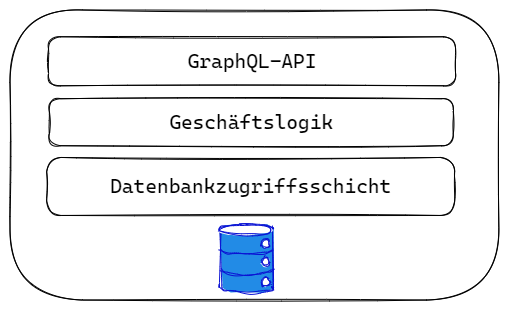
\includegraphics[width=\textwidth]{pics/architecture.png}
    \caption{Drei-Schicht-Architektur}
\end{figure}

Die hier abgebildete Architektur dient zur Veranschaulichung, die gezeigten Schichten werden in den folgenden Unterkapiteln genauer erklärt.

\subsection{API:}
Die API bildet die einzige Schnittstelle des Systems zur Außenwelt.
Sie wird mittels dem GraphQL-Schema abgebildet.
Dieses Schema definiert wie im GraphQL-Kapitel bereits erwähnt die verfügbaren Typen (Objekt-Typen, Input-Typen, ...) als auch die lesenden und schreibenden Zugriffe die der Service zur Verfügung stellt.

Bevor man sich als Entwickler an die Definition des Schemas heranwagt, sollte man zuallererst die Use-Cases, welche der Service zu erfüllen hat definieren.
Die Use-Cases, welcher der Prototyp zu erfüllen hat, sind in der folgenden Abbildung anschaulich dargestellt:

\begin{figure}[H]
    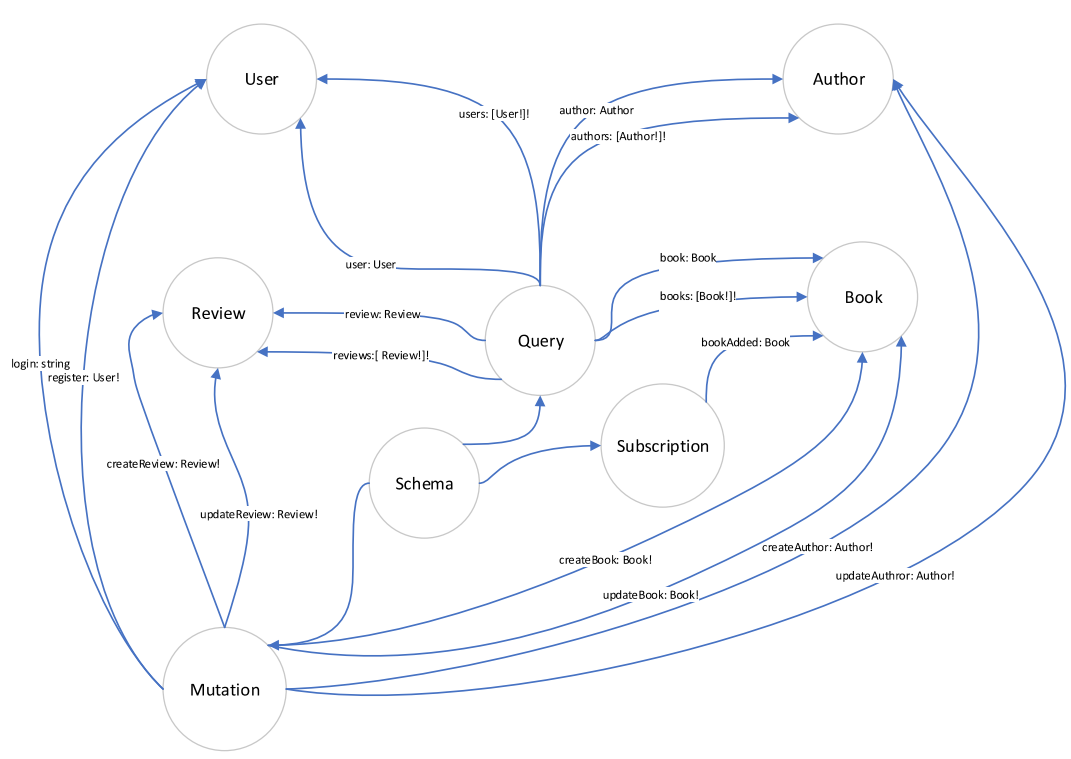
\includegraphics[width=\textwidth]{pics/graph_usecases.png}
    \caption{Use-Cases des Service.}
\end{figure}

In der Grafik ist das Schema anschaulich verdeutlicht.
Es zeigt das Schema und die Definierung der Wurzeloperationen für Query, Mutation und Subscription.
Weiters zeigt es die Operationen welche von den Queries, Mutations und Subscriptions auf die Entitäten abgebildet werden können.

Die Relationen zwischen den Entitäten sind im folgenden ER-Diagram dargestellt:
\begin{figure}[H]
    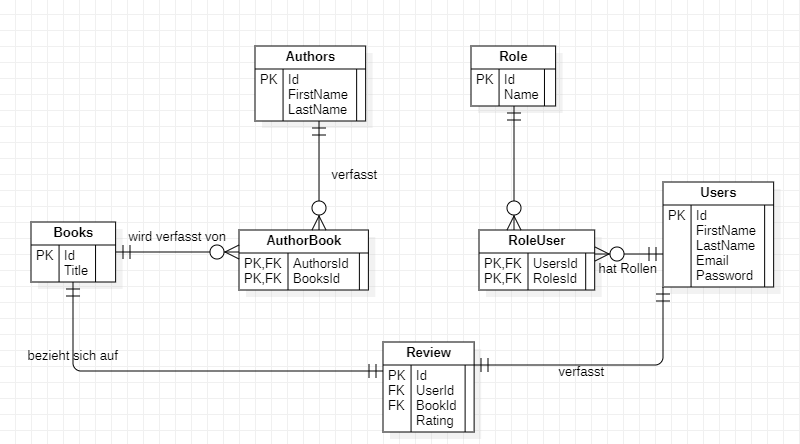
\includegraphics[width=\textwidth]{pics/ER-Diagram.png}
    \caption{Datenbankschema}
\end{figure}

\myparagraph{Definierung des Schemas mit HotChocolate}
% Die API die einzige Schnittstelle des Systems zur Außenwelt.
% \newline

\subsection{Geschäftslogik:}
Die Geschäftslogik bildet dabei die Logik der Server-Applikation ab.

GraphQL an sich ist gegliedert, oben ist die API darunter die Resolver, API selber (Schema) hat kein Wissen über das holen / schreiben der Daten sondern liefert nur Struktur.
Resolver kümmern sich um den Rest.
% \newline

\subsection{Datenbankzugriff:}
Die darunterliegende Datenbankzugriffsschicht ermöglicht, den darüberliegenden Schichten, CRUD-Operationen auf die angeforderten Daten auszuführen.
% \newline


\section{Hot Chocolate}
Der GraphQL-Service wurde mit dem Framework \textit{Hot Chocolate} umgesetzt.
Bei Hot Chocolate handelt es sich um einen Open Source GraphQL-Server welche 

\subsection{Entwurf Schema}

\section{Entity Framework}
Die Datenbankzugriffsschicht wurde mit dem \textit{Entity Framework} umgesetzt.
Das Entity Framework ist ein \textit{Object Relational Mapper}, es ermöglicht Entwicklern den Fokus auf eine höhere Abstraktionsebene zu legen.

\section{Resolver}
Das Schema beschreibt, wie bereits im GraphQL-Kapitel erwähnt, nur die verfügbaren Typen, Querys, Mutations und Subscriptions.
Über die Generierung der Daten als auch über die Manipulation derer hat das Schema kein Wissen.
Für den Datenzugriff bzw. Datenmanipulation sind in GraphQL \textit{Resolver} verantwortlich.
Jedes Feld in einer Query ist nichts anderes als eine Methode welches den Wert dieses Typs retourniert.
Jedes Feld eines Typs wird dabei einem \textit{Resolver} zugewiesen, diese Resolver sind Zugriffe auf die Geschäftslogik.
Wird ein Feld durch eine Query angefordert, liefert der jeweilige \textit{Resolver} die angeforderten Daten zurück.

\myparagraph{Umsetzung Resolver mittels Geschäftslogik}
Resolver werden im Prototypen durch die Geschäftslogik abgebildet, diese bieten CRUD-Operationen für die jeweilige Entität.
Jede Entität verfügt dabei über einen \textit{Service}.
Jeder Service wie zum Beispiel der \textit{AuthorService}, leitet dabei von einem generisch implementierten \textit{BaseService} ab.
Dieser \textit{BaseService} implementiert dabei das Interface \textit{BaseService}.
% Diese Services werden durch ein generisches \textit{Interface} \textit{IBaseService} und eine generische Basisimplementierung \textit{IBaseService} definiert.
\newline

\begin{JsCode}
public interface IBaseService<TEntity> where TEntity: BaseEntity {
    public Task<IQueryable<TEntity>> GetAsync(Expression<Func<TEntity, bool>> filter = null, params Expression<Func<TEntity, object>>[] includes);
    public Task<TEntity> GetFirstAsync(Expression<Func<TEntity, bool>> filter = null, params Expression<Func<TEntity, object>>[] includes);
    public Task<TEntity> AddAsync(TEntity entity);
    public Task<TEntity> UpdateAsync(TEntity entity);
    public Task<bool> ExistsAsync(int id);
    public Task RemoveAsync(TEntity entity);
}
\end{JsCode}

Im obigen CodeBeispiel ist das generische Interface \textit{IBaseService} abgebildet.
Es bietet Schnittstellen für die CRUD-Operationen jeder Entität.

\begin{JsCode}
public class BaseService<TEntity> : IBaseService<TEntity> where TEntity : BaseEntity {
    protected readonly IRepository<TEntity> repository;

    public BaseService(IRepository<TEntity> repository) {
        this.repository = repository;
    }
    public virtual async Task<IQueryable<TEntity>> GetAsync(Expression<Func<TEntity, bool>> filter = null, params Expression<Func<TEntity, object>>[] includes) {
        return await repository.GetAsync(filter, includes);
    }

    public virtual async Task<TEntity> GetFirstAsync(Expression<Func<TEntity, bool>> filter = null, params Expression<Func<TEntity, object>>[] includes) {
        return await repository.GetFirstAsync(filter, includes);
    }

    public virtual Task<TEntity> AddAsync(TEntity entity) {
        return repository.AddAsync(entity);
    }
    public virtual async Task<TEntity> UpdateAsync(TEntity entity) {
        return await repository.UpdateAsync(entity);
    }

    public virtual async Task<bool> ExistsAsync(int id) {
        return await repository.ExistsAsync(id);
    }

    public virtual async Task RemoveAsync(TEntity entity) {
        await repository.RemoveAsync(entity);
    }
}
\end{JsCode}

Im obigen Code-Beispiel ist die Basisimplementierung jedes Service zu sehen.
Besonders relevant für das Zusammenspiel mit HotChocolate ist dabei, dass die lesenden Operationen ein \textit{IQueryable} zurückliefern.
Warum \textit{IQueryable} so wichtig ist für HotChocolate wird im Abschnitt \textit{Projections} näher erläutert.
\newline

Zusammenfassend lassen sich Resolver wie folgt zusammenfassen: Sie bieten den angefragten Feldern die benötigte Logik der Geschäftslogik um eben jene abgefragten Felder bereitzustellen.

\section{Querys}
Im folgenden Abschnitt wird die Umsetzung eines lesenden Zugriffs mittels einer Query auf die Entität \textit{Book} erläutert.
Dabei wird das Zustandekommen der Schema-Definition der Query, als auch der Zugriff auf die Datenbank mittels der Geschäftslogik erläutert.
Weiters wird erläutert wie HotChocolate das Over und Underfetching Problem löst, als auch Filtern, Sortieren und Pagination ermöglicht.
\newline
Die folgenden Unterkapitel widmen sich der Umsetzung der Query \textit{authors} welche alle im System gespeicherten Autoren liefert.
Dabei kann man diese Entitäten filtern, sortieren und paginieren. %TODO --> paginieren nicht so nice i guess

\myparagraph{Generierung Schema}
Um es einem Client zu ermöglichen auf die Autoren zuzugreifen, ist es erforderlich die Query im Schema zu definieren.
Hierbei wird für die Generierung des Schemas, das bereits erwähnte Pure-Code-First verwendet.
\newline

\begin{JsCode}
public class AuthorQuery: ObjectType<Query> {
    protected override void Configure(IObjectTypeDescriptor<Query> descriptor) {
        descriptor.Field("authors")
            .ResolveWith<AuthorResolver>(r => r.Authors())
            .Authorize()
            .UseProjection()
            .UseFiltering()
            .UseSorting()
            .Type<ListType<NonNullType<AuthorType>>>();
    }
}
\end{JsCode}

Im obigen Code-Beispiel ist zu sehen, dass die Wurzeloperation \textit{Query} um eine \textit{AuthorQuery} erweitert wird.
Überschreibt man nun die in der Klasse \textit{ObjectType} definierte Methode \textit{Configure} kann man die Felder der Query mit dem \textit{IObjectTypeDescriptor} erweitern.
Dabei wird das Feld \textit{authors} angelegt welches eine Liste von Autoren zurückgibt.

Das obige Code-Beispiel generiert dabei zur Laufzeit die im nächsten Code-Beispiel gezeigte Query.
Dabei gilt zu erwähnen, dass nur der \textit{AuthorType} als auch die Wurzel-Operation der Query mit dem Feld \textit{authors} explizit generiert wird.
Alle anderen Typen wurden von HotChocolate implizit generiert.

\begin{JsCode}
type Query{
    authors(where: AuthorFilterInput order: [AuthorSortInput!]): [Author!] @authorize(apply: BEFORE_RESOLVER)
}

type Author {
    firstName: String!
    lastName: String!
    books: [Book!]!
    id: Int!
}

input AuthorFilterInput {
    and: [AuthorFilterInput!]
    or: [AuthorFilterInput!]
    firstName: StringOperationFilterInput
    lastName: StringOperationFilterInput
    books: ListFilterInputTypeOfBookFilterInput
    id: ComparableInt32OperationFilterInput
}

input ListFilterInputTypeOfBookFilterInput {
  all: BookFilterInput
  none: BookFilterInput
  some: BookFilterInput
  any: Boolean
}

input AuthorSortInput {
    firstName: SortEnumType
    lastName: SortEnumType
    id: SortEnumType
}

input StringOperationFilterInput {
  and: [StringOperationFilterInput!]
  or: [StringOperationFilterInput!]
  eq: String
  neq: String
  contains: String
  ncontains: String
  in: [String]
  nin: [String]
  startsWith: String
  nstartsWith: String
  endsWith: String
  nendsWith: String
}

input ComparableInt32OperationFilterInput {
    eq: Int
    neq: Int
    in: [Int!]
    nin: [Int!]
    gt: Int
    ngt: Int
    gte: Int
    ngte: Int
    lt: Int
    nlt: Int
    lte: Int
    nlte: Int
}
\end{JsCode}

%TODO Aufrufe relevant pagination -> projection -> filtering -> sorting
%todo die absätze aufeinander abstimmen erwähnen dass nur sortiert werden kann nachdem gefiltert wurde usw... bis nach oben hin
%sorting, filtering, projection ist ja nichts anders als middelware die nacheinander exekutiert wird, dabei Grafik von HotChocolate verwenden zur Veranschaulichung
\subsection{Field Middleware}
Die Methodenaufrufe \textit{Authorize()}, \textit{UseProjection()}, \textit{UseFiltering()} und \textit{UseSorting()} sind dabei für die Generierung von nicht explizit angegeben Typen verantwortlich.
Diese Methoden sind Field-Middleware Komponenten von HotChocolate.
Sie sind eine der fundamentalen Komponenten des Frameworks.
Field-Middleware erlaubt es, wiederverwendbare Logik vor oder nach der Exekution des Resolvers auszuführen.
Field-Middleware ist dabei \textit{composable}, somit kann man beliebig viele Middleware Komponenten aneinanderreihen.

\myparagraph{Reihenfolge Exekution Middleware}
Middlewarekomponenten werden in der Reihenfolge in der sie definiert worden sind ausgeführt.
Jede Middleware-Schicht kennt dabei nur die jeweils nächste Middleware.
Die letzte auszuführende Middleware ist dabei der eigentliche Resolver.
Die Reihenfolge der Anordnung der Middlewarekomponenten ist dabei sehr entscheidend, denn die Komponenten werden in genau dieser Reihenfolge exekutiert.
% Die Reihenfolge in der diese Middlewarekomponenten ausgeführt werden ist dabei sehr wichtig, denn sie entscheidet in welcher 
Die folgende Abbildung beschreibt die Aneinanderreihung der Middlewarekomponenten:

\begin{figure}[H]
    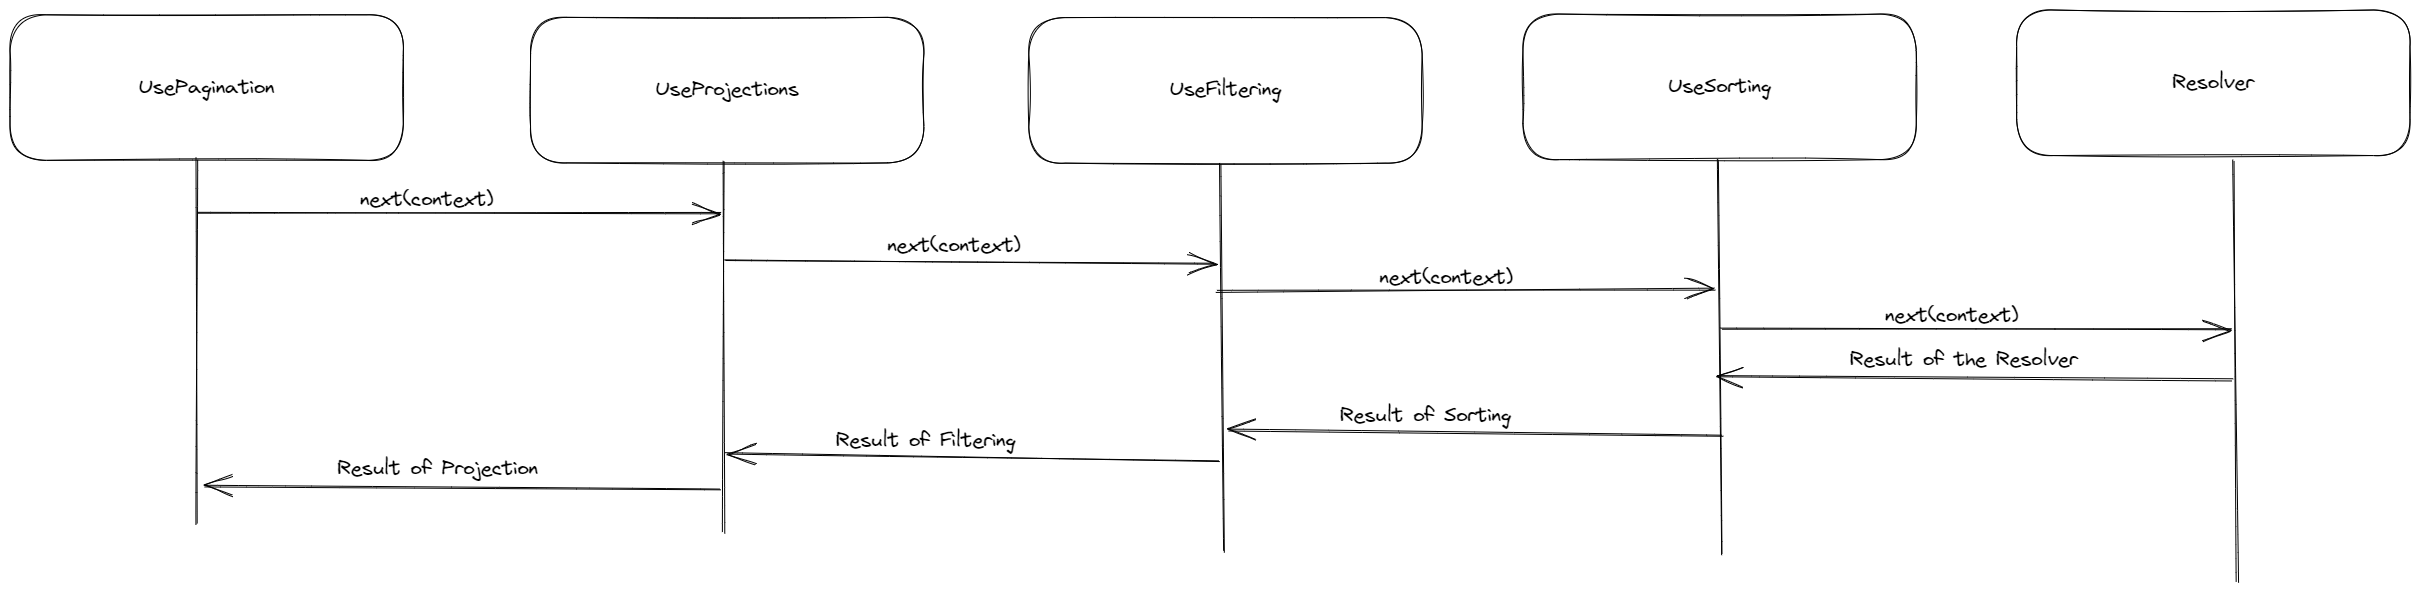
\includegraphics[width=\textwidth]{pics/middleware.png}
    \caption{Exekutierungsreihenfolge Middleware}
\end{figure}

In der obigen Abbildung ist zu sehen, dass die Middleware in der Reihenfolge ausgeführt wird in der sie definiert wurde.
Aber das Resultat welches von der letzten Middleware (dem Resolver) generiert wurde, wird in der umgekehrten Reihenfolge zurückgereicht.
Dabei wird das vom Resolver zurückgelieferte \textit{IQueryable} um die jeweiligen Operationen der restlichen Middleware erweitert.
In den folgenden Abschnitten wird auf die verwendeten Middlewarekomponenten genauer eingegangen: 

\myparagraph{Authorize}
Hierbei wird deklariert, dass nur angemeldete Benutzer Zugriff auf diese Query haben.
Diese Middleware, ist wie in der obigen Schemadefinition ersichtlich, vor dem Resolver auszuführen.
Sie stellt damit sicher, dass nur Anfragen mit einer gültigen Authentifizierung ausgeführt werden.
Im Schema wird das Feld \textit{authors} der Query mit der Direktive \textit{@authorize} versehen.
Näheres zur Authentifizierung und Autorisierung ist im gleichnamigen Abschnitt ersichtlich.

\myparagraph{Projection}
Mit \textit{Projections} liefert HotChocolate die Möglichkeit Over und Underfetching zu verhindern.
Over und Underfetching zu verhindern bedeutet, dass genau jene Daten, welche vom Client angefordert werden, in der Datenbank selektiert und anschließend an den Client zurückgeliefert werden.
Dabei bekommt HotChocolate vom \textit{Resolver} ein \textit{IQueryable}.
Dieses \textit{IQueryable} beinhaltet zunächst nur jene Filterungen und Selektionen welche von der Geschäftslogik festgelegt worden sind.
HotChocolate erweitert dieses \textit{IQueryable} nun durch jene Felder welche in der Query angefordert wurden.

\myparagraph{Filtering}
Aktiviert man die \textit{Filtering} Middleware für ein Query-Field so kann man den implizit von HotChocolate bereitgestellten Sortier-Input verwenden.
Diese Middleware erweitert das vom Resolver zurückgelieferte \textit{IQueryable} um die gegebene Filterung und liefert das Ergebnis der vorangestellten Middleware zurück.

\myparagraph{Sorting}
% Aktiviert man die \textit{Sorting} Middleware für ein Query-Field so kann man entweder selbst einen Sortier-Input definieren, oder den implizit von HotChocolate bereitgestellten Sortier-Input verwenden.


\myparagraph{Ausführung Query und Ergebnis}

\myparagraph{Generiertes SQL-Statement}

\begin{JsCode}
builder.Services
    .AddGraphQLServer()
    .AddAuthorization()
    .AddProjections()
    .AddFiltering()
    .AddSorting()
    .AddQueryType<Query>()
    .AddTypeExtension<AuthorQuery>();
\end{JsCode}

\section{Mutations}

\section{Subscriptions}

\section{Authentifizierung und Autorisierung}

\begin{figure}[H]
    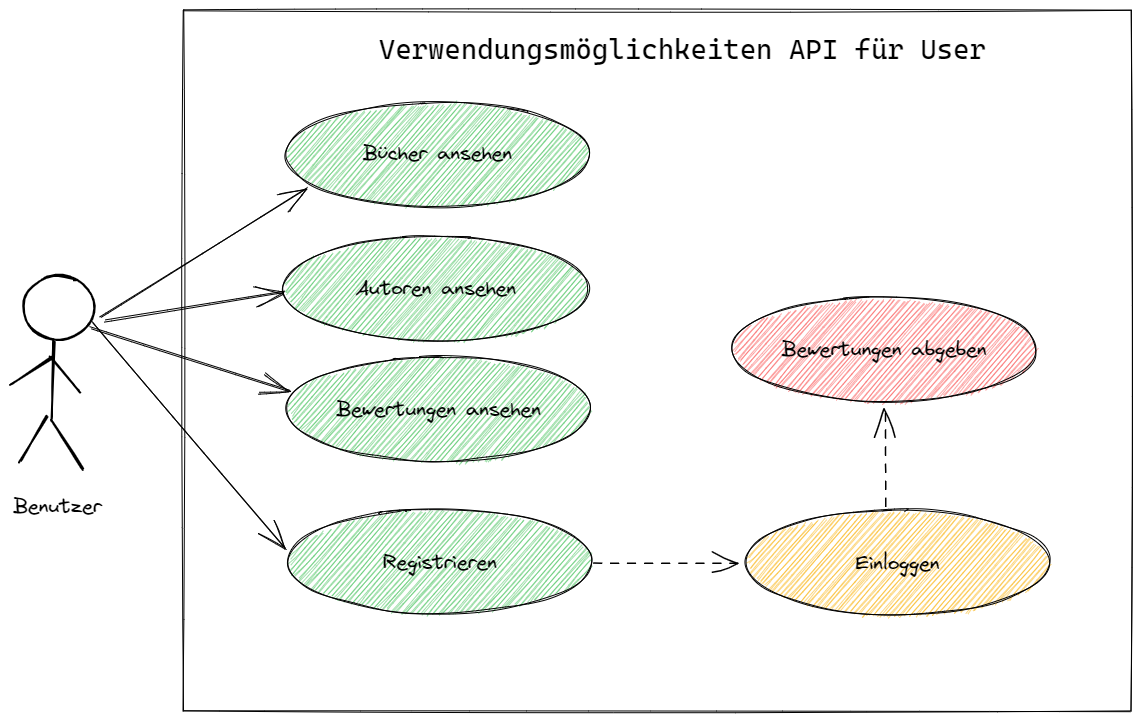
\includegraphics[width=\textwidth]{pics/UseCaseUser.png}
    \caption{Rechte User.}
\end{figure}

\begin{figure}[H]
    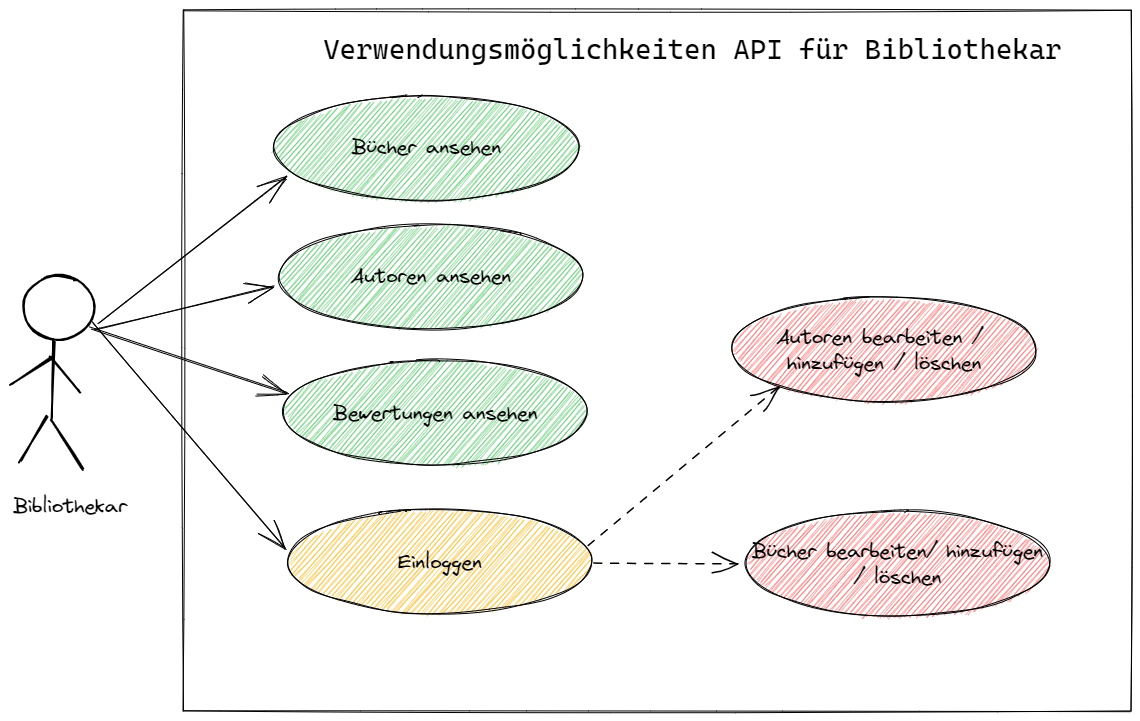
\includegraphics[width=\textwidth]{pics/UseCaseLibrarian.png}
    \caption{Rechte Bibliothekar.}
\end{figure}

\begin{figure}[H]
    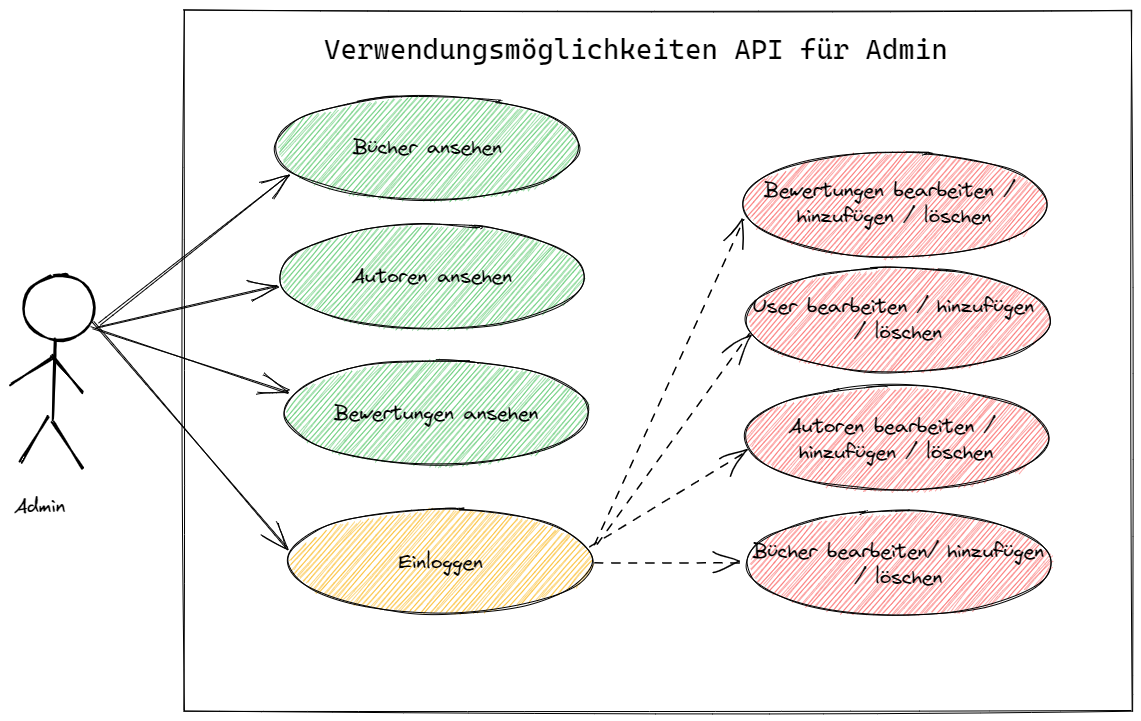
\includegraphics[width=\textwidth]{pics/UseCaseAdmin.png}
    \caption{Rechte Admin.}
\end{figure}

\section{1 + n Problem}
Lösung mit Dataloader
\section{Entwicklertools}
\subsection{GraphiQL}

